% Options for packages loaded elsewhere
\PassOptionsToPackage{unicode}{hyperref}
\PassOptionsToPackage{hyphens}{url}
\PassOptionsToPackage{dvipsnames,svgnames,x11names}{xcolor}
%
\documentclass[
  letterpaper,
  DIV=11,
  numbers=noendperiod]{scrartcl}

\usepackage{amsmath,amssymb}
\usepackage{iftex}
\ifPDFTeX
  \usepackage[T1]{fontenc}
  \usepackage[utf8]{inputenc}
  \usepackage{textcomp} % provide euro and other symbols
\else % if luatex or xetex
  \usepackage{unicode-math}
  \defaultfontfeatures{Scale=MatchLowercase}
  \defaultfontfeatures[\rmfamily]{Ligatures=TeX,Scale=1}
\fi
\usepackage{lmodern}
\ifPDFTeX\else  
    % xetex/luatex font selection
\fi
% Use upquote if available, for straight quotes in verbatim environments
\IfFileExists{upquote.sty}{\usepackage{upquote}}{}
\IfFileExists{microtype.sty}{% use microtype if available
  \usepackage[]{microtype}
  \UseMicrotypeSet[protrusion]{basicmath} % disable protrusion for tt fonts
}{}
\makeatletter
\@ifundefined{KOMAClassName}{% if non-KOMA class
  \IfFileExists{parskip.sty}{%
    \usepackage{parskip}
  }{% else
    \setlength{\parindent}{0pt}
    \setlength{\parskip}{6pt plus 2pt minus 1pt}}
}{% if KOMA class
  \KOMAoptions{parskip=half}}
\makeatother
\usepackage{xcolor}
\setlength{\emergencystretch}{3em} % prevent overfull lines
\setcounter{secnumdepth}{-\maxdimen} % remove section numbering
% Make \paragraph and \subparagraph free-standing
\ifx\paragraph\undefined\else
  \let\oldparagraph\paragraph
  \renewcommand{\paragraph}[1]{\oldparagraph{#1}\mbox{}}
\fi
\ifx\subparagraph\undefined\else
  \let\oldsubparagraph\subparagraph
  \renewcommand{\subparagraph}[1]{\oldsubparagraph{#1}\mbox{}}
\fi

\usepackage{color}
\usepackage{fancyvrb}
\newcommand{\VerbBar}{|}
\newcommand{\VERB}{\Verb[commandchars=\\\{\}]}
\DefineVerbatimEnvironment{Highlighting}{Verbatim}{commandchars=\\\{\}}
% Add ',fontsize=\small' for more characters per line
\usepackage{framed}
\definecolor{shadecolor}{RGB}{241,243,245}
\newenvironment{Shaded}{\begin{snugshade}}{\end{snugshade}}
\newcommand{\AlertTok}[1]{\textcolor[rgb]{0.68,0.00,0.00}{#1}}
\newcommand{\AnnotationTok}[1]{\textcolor[rgb]{0.37,0.37,0.37}{#1}}
\newcommand{\AttributeTok}[1]{\textcolor[rgb]{0.40,0.45,0.13}{#1}}
\newcommand{\BaseNTok}[1]{\textcolor[rgb]{0.68,0.00,0.00}{#1}}
\newcommand{\BuiltInTok}[1]{\textcolor[rgb]{0.00,0.23,0.31}{#1}}
\newcommand{\CharTok}[1]{\textcolor[rgb]{0.13,0.47,0.30}{#1}}
\newcommand{\CommentTok}[1]{\textcolor[rgb]{0.37,0.37,0.37}{#1}}
\newcommand{\CommentVarTok}[1]{\textcolor[rgb]{0.37,0.37,0.37}{\textit{#1}}}
\newcommand{\ConstantTok}[1]{\textcolor[rgb]{0.56,0.35,0.01}{#1}}
\newcommand{\ControlFlowTok}[1]{\textcolor[rgb]{0.00,0.23,0.31}{#1}}
\newcommand{\DataTypeTok}[1]{\textcolor[rgb]{0.68,0.00,0.00}{#1}}
\newcommand{\DecValTok}[1]{\textcolor[rgb]{0.68,0.00,0.00}{#1}}
\newcommand{\DocumentationTok}[1]{\textcolor[rgb]{0.37,0.37,0.37}{\textit{#1}}}
\newcommand{\ErrorTok}[1]{\textcolor[rgb]{0.68,0.00,0.00}{#1}}
\newcommand{\ExtensionTok}[1]{\textcolor[rgb]{0.00,0.23,0.31}{#1}}
\newcommand{\FloatTok}[1]{\textcolor[rgb]{0.68,0.00,0.00}{#1}}
\newcommand{\FunctionTok}[1]{\textcolor[rgb]{0.28,0.35,0.67}{#1}}
\newcommand{\ImportTok}[1]{\textcolor[rgb]{0.00,0.46,0.62}{#1}}
\newcommand{\InformationTok}[1]{\textcolor[rgb]{0.37,0.37,0.37}{#1}}
\newcommand{\KeywordTok}[1]{\textcolor[rgb]{0.00,0.23,0.31}{#1}}
\newcommand{\NormalTok}[1]{\textcolor[rgb]{0.00,0.23,0.31}{#1}}
\newcommand{\OperatorTok}[1]{\textcolor[rgb]{0.37,0.37,0.37}{#1}}
\newcommand{\OtherTok}[1]{\textcolor[rgb]{0.00,0.23,0.31}{#1}}
\newcommand{\PreprocessorTok}[1]{\textcolor[rgb]{0.68,0.00,0.00}{#1}}
\newcommand{\RegionMarkerTok}[1]{\textcolor[rgb]{0.00,0.23,0.31}{#1}}
\newcommand{\SpecialCharTok}[1]{\textcolor[rgb]{0.37,0.37,0.37}{#1}}
\newcommand{\SpecialStringTok}[1]{\textcolor[rgb]{0.13,0.47,0.30}{#1}}
\newcommand{\StringTok}[1]{\textcolor[rgb]{0.13,0.47,0.30}{#1}}
\newcommand{\VariableTok}[1]{\textcolor[rgb]{0.07,0.07,0.07}{#1}}
\newcommand{\VerbatimStringTok}[1]{\textcolor[rgb]{0.13,0.47,0.30}{#1}}
\newcommand{\WarningTok}[1]{\textcolor[rgb]{0.37,0.37,0.37}{\textit{#1}}}

\providecommand{\tightlist}{%
  \setlength{\itemsep}{0pt}\setlength{\parskip}{0pt}}\usepackage{longtable,booktabs,array}
\usepackage{calc} % for calculating minipage widths
% Correct order of tables after \paragraph or \subparagraph
\usepackage{etoolbox}
\makeatletter
\patchcmd\longtable{\par}{\if@noskipsec\mbox{}\fi\par}{}{}
\makeatother
% Allow footnotes in longtable head/foot
\IfFileExists{footnotehyper.sty}{\usepackage{footnotehyper}}{\usepackage{footnote}}
\makesavenoteenv{longtable}
\usepackage{graphicx}
\makeatletter
\def\maxwidth{\ifdim\Gin@nat@width>\linewidth\linewidth\else\Gin@nat@width\fi}
\def\maxheight{\ifdim\Gin@nat@height>\textheight\textheight\else\Gin@nat@height\fi}
\makeatother
% Scale images if necessary, so that they will not overflow the page
% margins by default, and it is still possible to overwrite the defaults
% using explicit options in \includegraphics[width, height, ...]{}
\setkeys{Gin}{width=\maxwidth,height=\maxheight,keepaspectratio}
% Set default figure placement to htbp
\makeatletter
\def\fps@figure{htbp}
\makeatother

\KOMAoption{captions}{tableheading}
\makeatletter
\makeatother
\makeatletter
\makeatother
\makeatletter
\@ifpackageloaded{caption}{}{\usepackage{caption}}
\AtBeginDocument{%
\ifdefined\contentsname
  \renewcommand*\contentsname{Table of contents}
\else
  \newcommand\contentsname{Table of contents}
\fi
\ifdefined\listfigurename
  \renewcommand*\listfigurename{List of Figures}
\else
  \newcommand\listfigurename{List of Figures}
\fi
\ifdefined\listtablename
  \renewcommand*\listtablename{List of Tables}
\else
  \newcommand\listtablename{List of Tables}
\fi
\ifdefined\figurename
  \renewcommand*\figurename{Figure}
\else
  \newcommand\figurename{Figure}
\fi
\ifdefined\tablename
  \renewcommand*\tablename{Table}
\else
  \newcommand\tablename{Table}
\fi
}
\@ifpackageloaded{float}{}{\usepackage{float}}
\floatstyle{ruled}
\@ifundefined{c@chapter}{\newfloat{codelisting}{h}{lop}}{\newfloat{codelisting}{h}{lop}[chapter]}
\floatname{codelisting}{Listing}
\newcommand*\listoflistings{\listof{codelisting}{List of Listings}}
\makeatother
\makeatletter
\@ifpackageloaded{caption}{}{\usepackage{caption}}
\@ifpackageloaded{subcaption}{}{\usepackage{subcaption}}
\makeatother
\makeatletter
\@ifpackageloaded{tcolorbox}{}{\usepackage[skins,breakable]{tcolorbox}}
\makeatother
\makeatletter
\@ifundefined{shadecolor}{\definecolor{shadecolor}{rgb}{.97, .97, .97}}
\makeatother
\makeatletter
\makeatother
\makeatletter
\makeatother
\ifLuaTeX
  \usepackage{selnolig}  % disable illegal ligatures
\fi
\IfFileExists{bookmark.sty}{\usepackage{bookmark}}{\usepackage{hyperref}}
\IfFileExists{xurl.sty}{\usepackage{xurl}}{} % add URL line breaks if available
\urlstyle{same} % disable monospaced font for URLs
\hypersetup{
  pdftitle={STAT 118: Notes J},
  pdfauthor={Emily Malcolm-White},
  colorlinks=true,
  linkcolor={blue},
  filecolor={Maroon},
  citecolor={Blue},
  urlcolor={Blue},
  pdfcreator={LaTeX via pandoc}}

\title{STAT 118: Notes J}
\usepackage{etoolbox}
\makeatletter
\providecommand{\subtitle}[1]{% add subtitle to \maketitle
  \apptocmd{\@title}{\par {\large #1 \par}}{}{}
}
\makeatother
\subtitle{\texttt{tidyr}: reshaping data with \texttt{pivot\_longer()}
and \texttt{pivot\_wider()}\\

\includegraphics[width=0.1\textwidth,height=\textheight]{118_J_pivoting_Notes_files/mediabag/logo.png}}
\author{Emily Malcolm-White}
\date{}

\begin{document}
\maketitle
\ifdefined\Shaded\renewenvironment{Shaded}{\begin{tcolorbox}[enhanced, frame hidden, breakable, interior hidden, boxrule=0pt, sharp corners, borderline west={3pt}{0pt}{shadecolor}]}{\end{tcolorbox}}\fi

\includegraphics{118_J_pivoting_Notes_files/mediabag/ross-pivot-friends.gif}

\hypertarget{reshaping-with-pivoting-why}{%
\section{Reshaping with Pivoting --
Why?}\label{reshaping-with-pivoting-why}}

Data frames are often described as wide or long.

\emph{Wide} when a row has more than one observation, and the units of
observation are on one row each

\emph{Long} when a row has only one observation, but the units of
observation are repeated down the column

\begin{figure}

{\centering 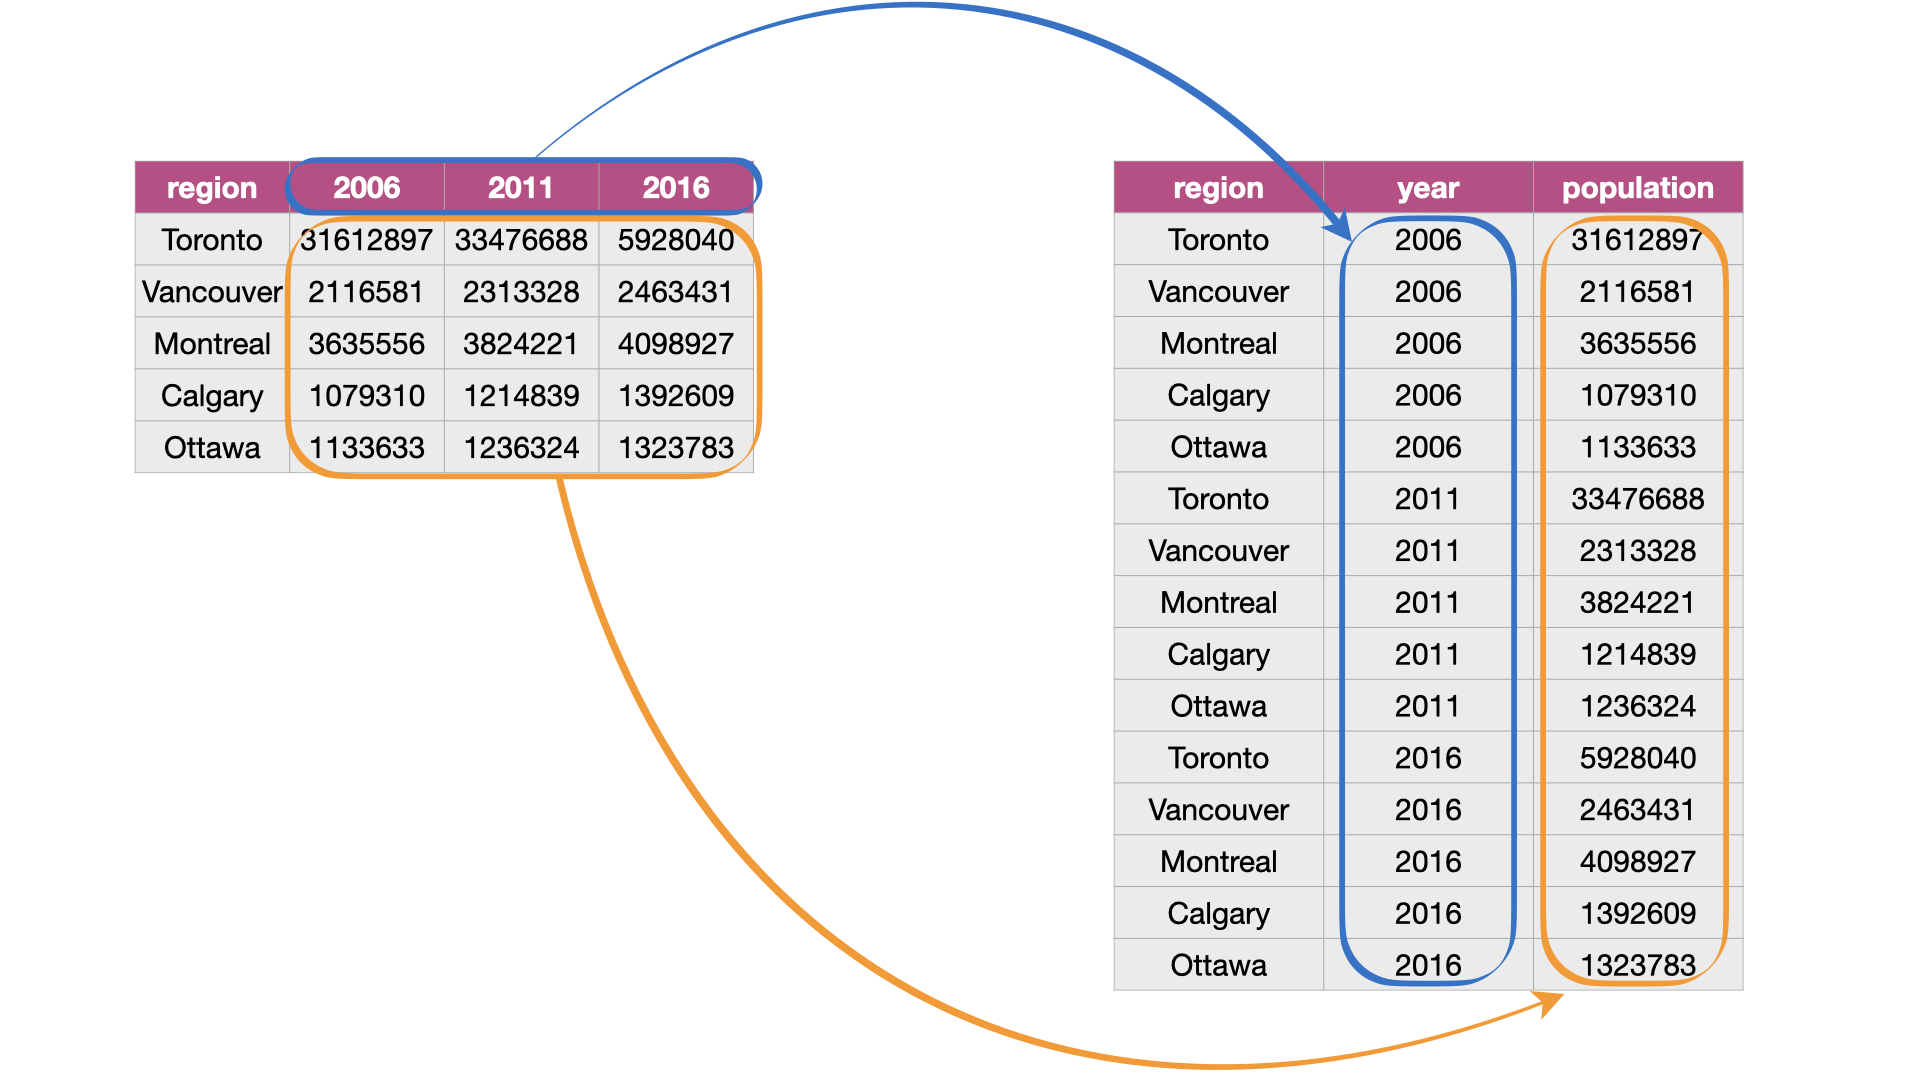
\includegraphics{118_J_pivoting_Notes_files/mediabag/pivot_functions.001.jpg}

}

\caption{Credit: datasciencebook.ca}

\end{figure}

\hypertarget{canlang-dataset}{%
\section{\texorpdfstring{\texttt{canlang}
dataset}{canlang dataset}}\label{canlang-dataset}}

\begin{Shaded}
\begin{Highlighting}[]
\CommentTok{\#LOAD PACKAGES}
\FunctionTok{library}\NormalTok{(tidyverse)}

\CommentTok{\#LOAD DATA}
\NormalTok{lang\_wide }\OtherTok{\textless{}{-}} \FunctionTok{read.csv}\NormalTok{(}\StringTok{"https://raw.githubusercontent.com/UBC{-}DSCI/introduction{-}to{-}datascience/master/data/region\_lang\_top5\_cities\_wide.csv"}\NormalTok{)}
\end{Highlighting}
\end{Shaded}

\hypertarget{pivot-longer}{%
\section{Pivot Longer}\label{pivot-longer}}

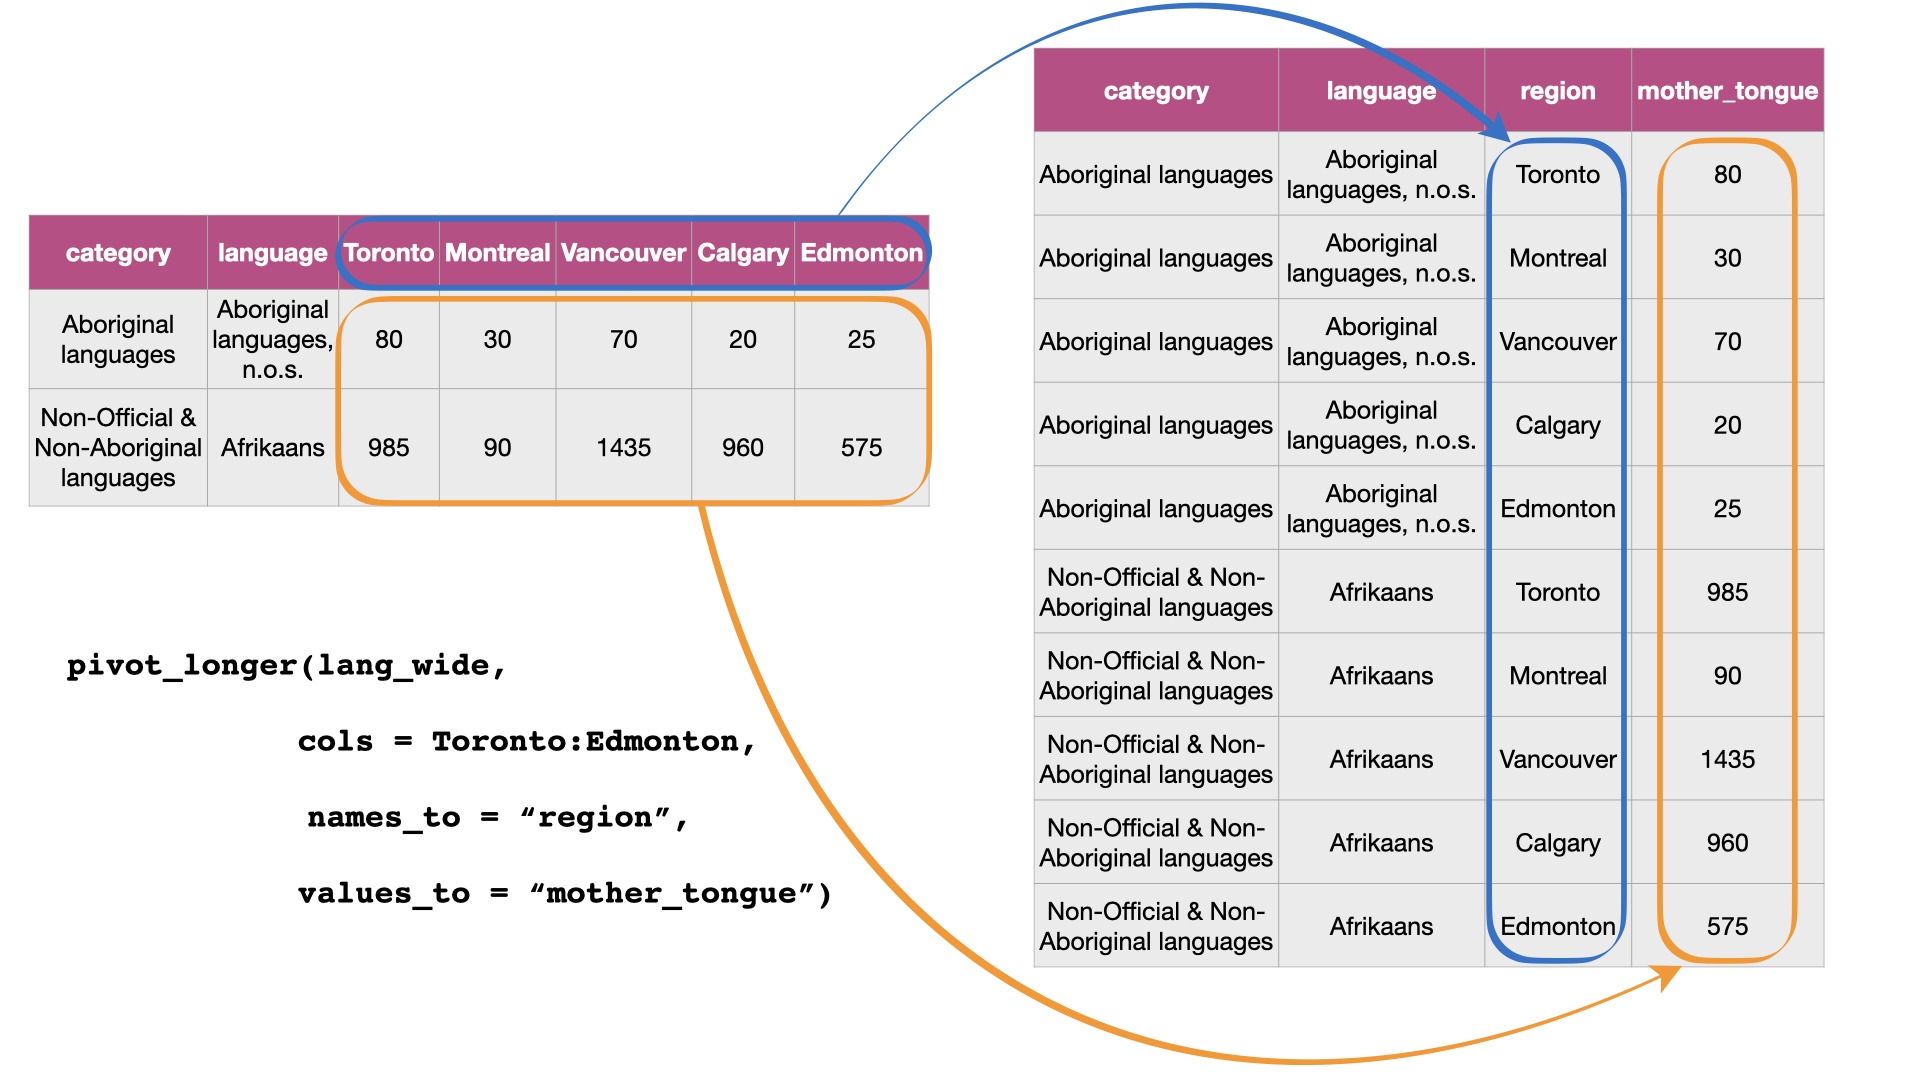
\includegraphics{118_J_pivoting_Notes_files/mediabag/pivot_functions.003.jpg}
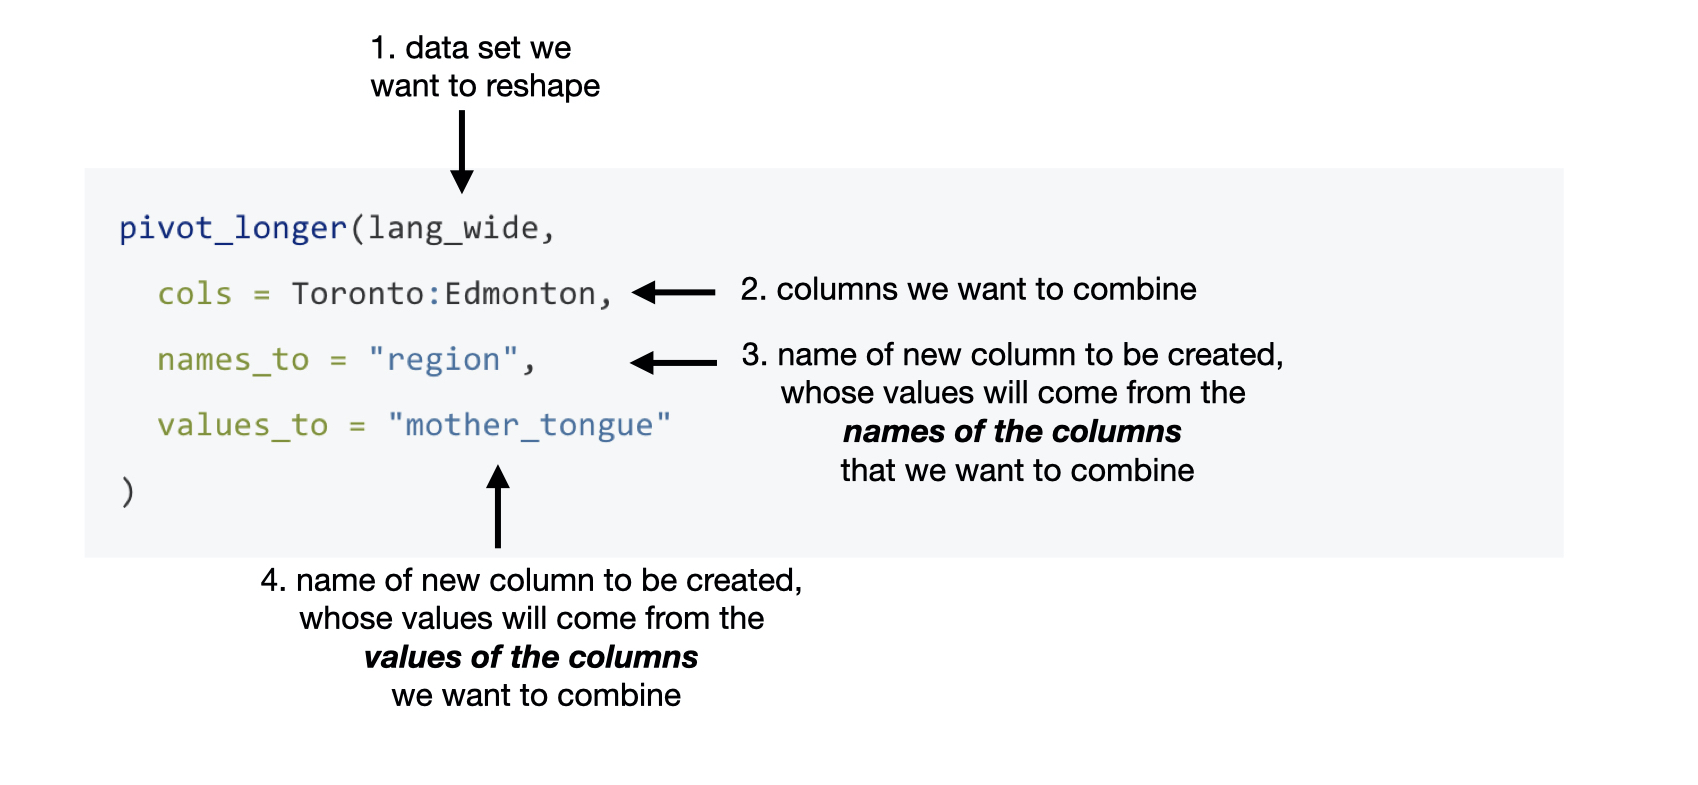
\includegraphics{118_J_pivoting_Notes_files/mediabag/pivot_longer.jpg}

\begin{Shaded}
\begin{Highlighting}[]
\NormalTok{lang\_mother\_tidy }\OtherTok{\textless{}{-}} \FunctionTok{pivot\_longer}\NormalTok{(lang\_wide,}
  \AttributeTok{cols =}\NormalTok{ Toronto}\SpecialCharTok{:}\NormalTok{Edmonton,}
  \AttributeTok{names\_to =} \StringTok{"region"}\NormalTok{,}
  \AttributeTok{values\_to =} \StringTok{"mother\_tongue"}
\NormalTok{)}

\NormalTok{lang\_mother\_tidy}
\end{Highlighting}
\end{Shaded}

\begin{verbatim}
# A tibble: 1,070 x 4
   category                                language         region mother_tongue
   <chr>                                   <chr>            <chr>          <int>
 1 Aboriginal languages                    Aboriginal lang~ Toron~            80
 2 Aboriginal languages                    Aboriginal lang~ Montr~            30
 3 Aboriginal languages                    Aboriginal lang~ Vanco~            70
 4 Aboriginal languages                    Aboriginal lang~ Calga~            20
 5 Aboriginal languages                    Aboriginal lang~ Edmon~            25
 6 Non-Official & Non-Aboriginal languages Afrikaans        Toron~           985
 7 Non-Official & Non-Aboriginal languages Afrikaans        Montr~            90
 8 Non-Official & Non-Aboriginal languages Afrikaans        Vanco~          1435
 9 Non-Official & Non-Aboriginal languages Afrikaans        Calga~           960
10 Non-Official & Non-Aboriginal languages Afrikaans        Edmon~           575
# i 1,060 more rows
\end{verbatim}

The data above is now tidy because all three criteria for tidy data have
now been met:

\begin{itemize}
\tightlist
\item
  All the variables (category, language, region and mother\_tongue) are
  now their own columns in the data frame.
\item
  Each observation, (i.e., each language in a region) is in a single
  row.
\item
  Each value is a single cell, i.e., its row, column position in the
  data frame is not shared with another value.
\end{itemize}

\hypertarget{pivot-wider}{%
\section{Pivot Wider}\label{pivot-wider}}

\begin{Shaded}
\begin{Highlighting}[]
\NormalTok{lang\_long }\OtherTok{\textless{}{-}} \FunctionTok{read.csv}\NormalTok{(}\StringTok{"https://raw.githubusercontent.com/UBC{-}DSCI/introduction{-}to{-}datascience/master/data/region\_lang\_top5\_cities\_long.csv"}\NormalTok{)}
\end{Highlighting}
\end{Shaded}

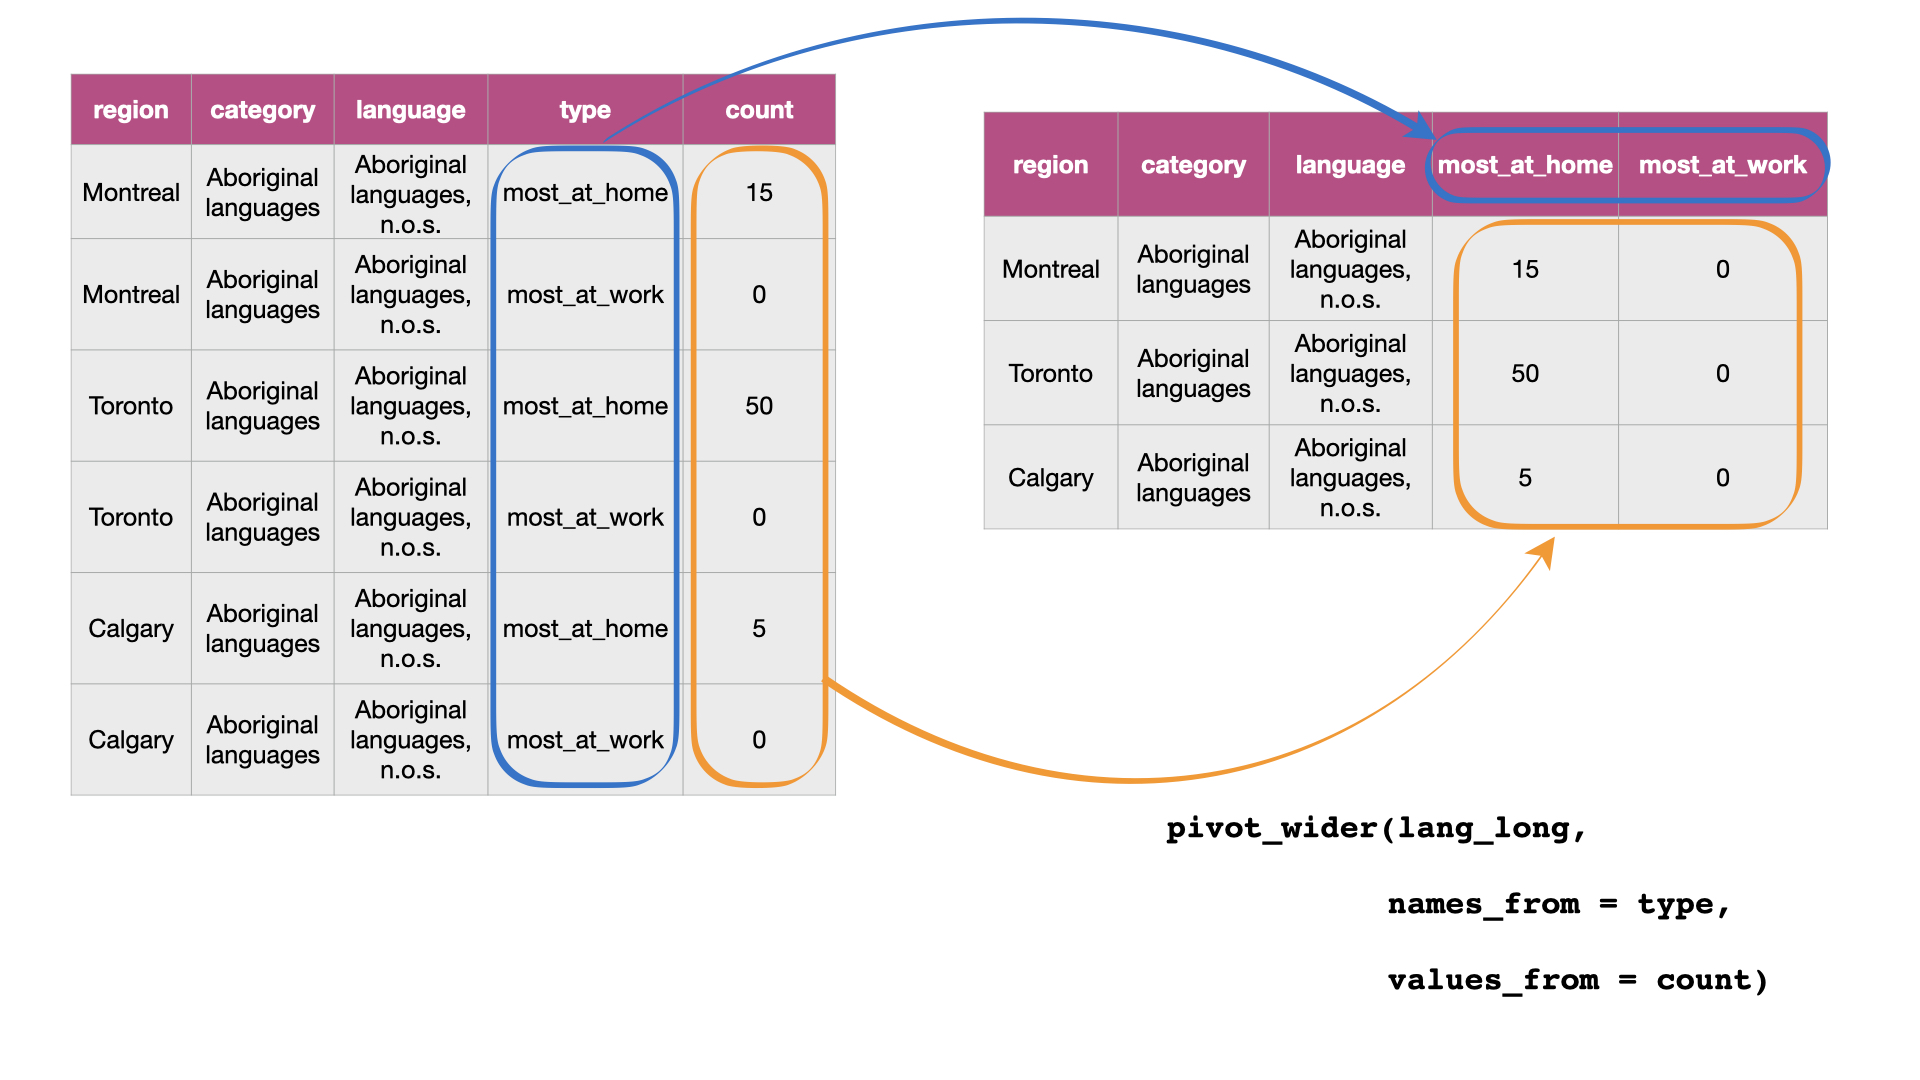
\includegraphics{118_J_pivoting_Notes_files/mediabag/pivot_functions.004.jpg}
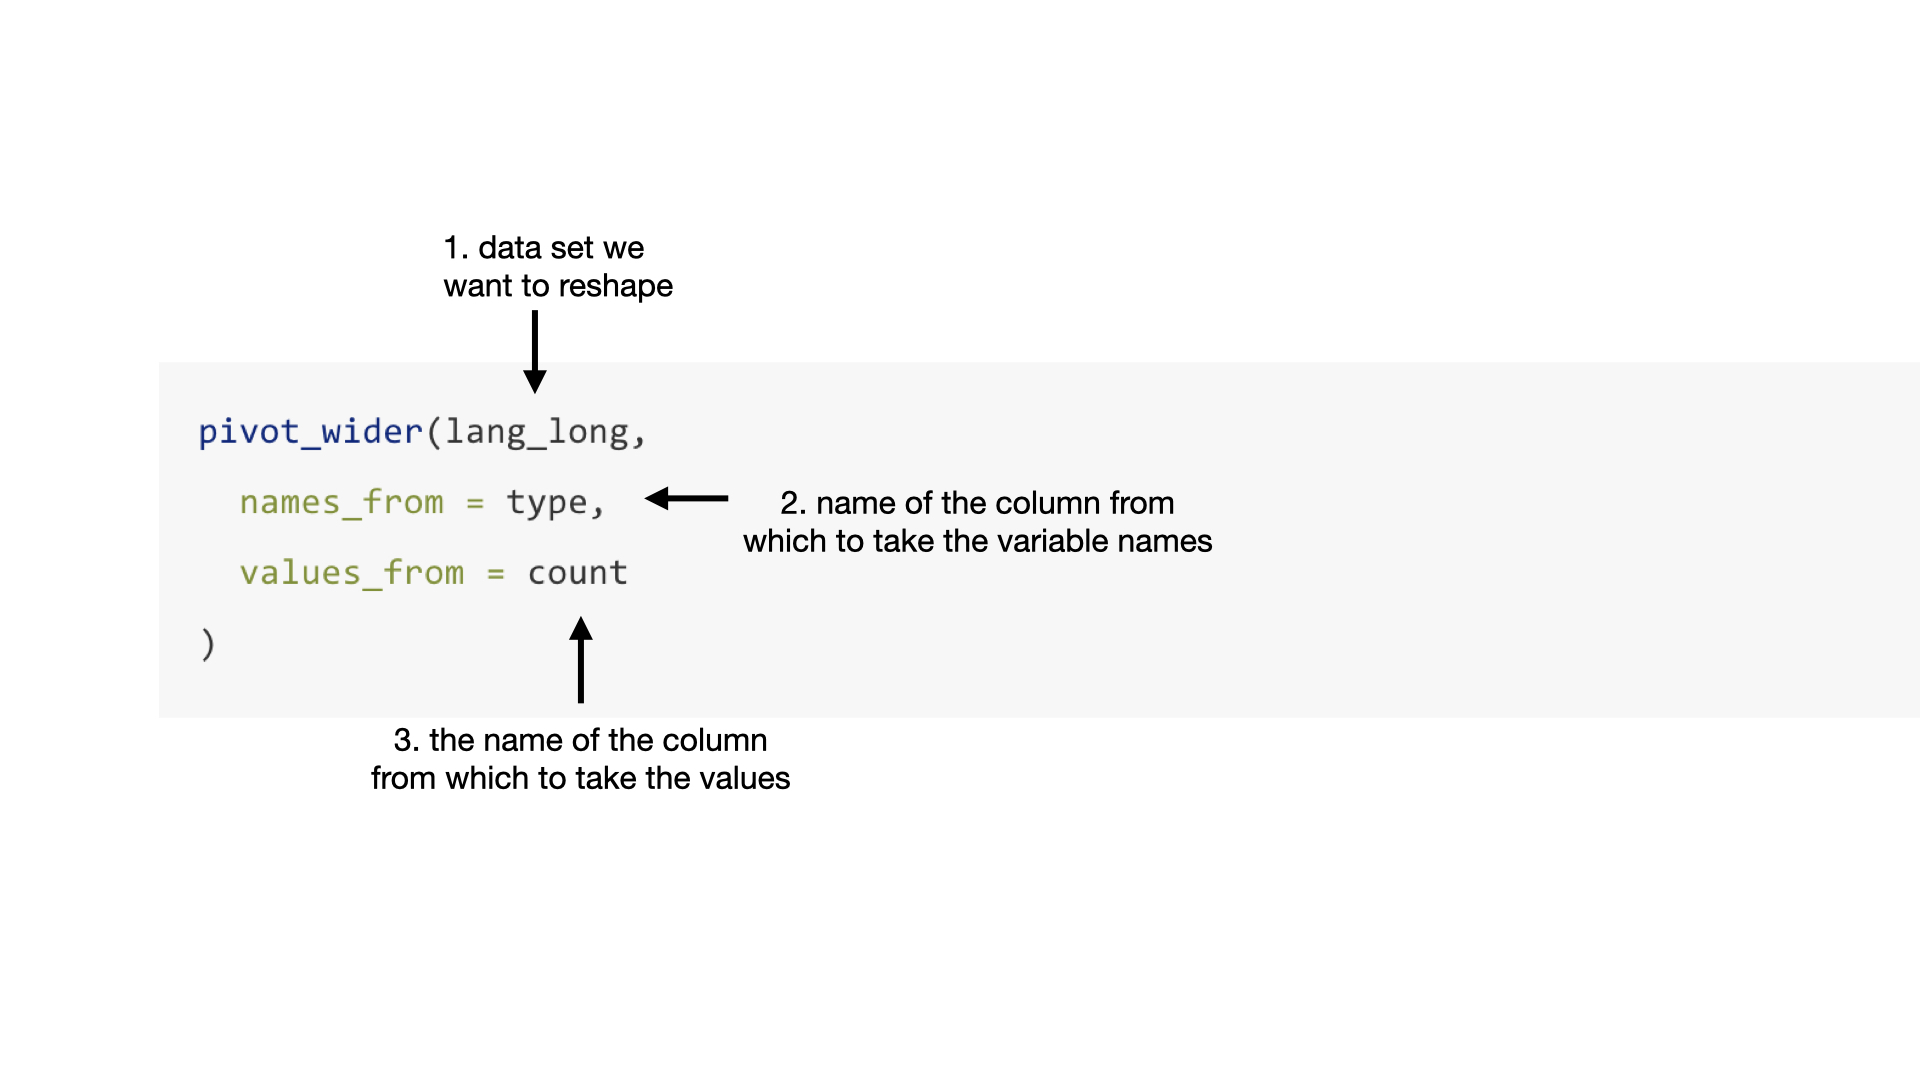
\includegraphics{118_J_pivoting_Notes_files/mediabag/pivot_wider.jpg}

\begin{Shaded}
\begin{Highlighting}[]
\NormalTok{lang\_home\_tidy }\OtherTok{\textless{}{-}} \FunctionTok{pivot\_wider}\NormalTok{(lang\_long,}
  \AttributeTok{names\_from =}\NormalTok{ type,}
  \AttributeTok{values\_from =}\NormalTok{ count}
\NormalTok{)}
\NormalTok{lang\_home\_tidy}
\end{Highlighting}
\end{Shaded}

\begin{verbatim}
# A tibble: 1,070 x 5
   region    category                         language most_at_home most_at_work
   <chr>     <chr>                            <chr>           <int>        <int>
 1 Montréal  Aboriginal languages             Aborigi~           15            0
 2 Toronto   Aboriginal languages             Aborigi~           50            0
 3 Calgary   Aboriginal languages             Aborigi~            5            0
 4 Edmonton  Aboriginal languages             Aborigi~           10            0
 5 Vancouver Aboriginal languages             Aborigi~           15            0
 6 Montréal  Non-Official & Non-Aboriginal l~ Afrikaa~           10            0
 7 Toronto   Non-Official & Non-Aboriginal l~ Afrikaa~          265            0
 8 Calgary   Non-Official & Non-Aboriginal l~ Afrikaa~          505           15
 9 Edmonton  Non-Official & Non-Aboriginal l~ Afrikaa~          300            0
10 Vancouver Non-Official & Non-Aboriginal l~ Afrikaa~          520           10
# i 1,060 more rows
\end{verbatim}

\hypertarget{gapminder}{%
\section{Gapminder}\label{gapminder}}

\begin{Shaded}
\begin{Highlighting}[]
\FunctionTok{library}\NormalTok{(gapminder)}
\FunctionTok{data}\NormalTok{(}\StringTok{"gapminder"}\NormalTok{)}
\end{Highlighting}
\end{Shaded}

Let's say we'd like to look at \texttt{LifeExp} over time for all the
countries in Asia in our dataset.

\begin{Shaded}
\begin{Highlighting}[]
\CommentTok{\# Create a dataset called asia with the data we need}
\NormalTok{asia }\OtherTok{\textless{}{-}}\NormalTok{ gapminder }\SpecialCharTok{\%\textgreater{}\%} 
  \FunctionTok{filter}\NormalTok{(continent }\SpecialCharTok{==} \StringTok{"Asia"}\NormalTok{) }\SpecialCharTok{\%\textgreater{}\%} 
  \FunctionTok{select}\NormalTok{(country, year, lifeExp)}
\end{Highlighting}
\end{Shaded}

We can create a wide version of our table, where each row is a country
and each column a year, with values of \texttt{lifeExp} in each cell of
the table.

\begin{Shaded}
\begin{Highlighting}[]
\NormalTok{lifeExp\_wide }\OtherTok{\textless{}{-}}\NormalTok{ asia }\SpecialCharTok{\%\textgreater{}\%} 
  \CommentTok{\# use pivot\_wider to go from long to wide format}
  \FunctionTok{pivot\_wider}\NormalTok{(}\AttributeTok{names\_from =} \StringTok{"year"}\NormalTok{, }
              \AttributeTok{names\_prefix =} \StringTok{"yr"}\NormalTok{, }\CommentTok{\#it’s a good idea to avoid column names that start with a number}
              \AttributeTok{values\_from =} \StringTok{"lifeExp"}\NormalTok{)}
\NormalTok{lifeExp\_wide}
\end{Highlighting}
\end{Shaded}

\begin{verbatim}
# A tibble: 33 x 13
   country yr1952 yr1957 yr1962 yr1967 yr1972 yr1977 yr1982 yr1987 yr1992 yr1997
   <fct>    <dbl>  <dbl>  <dbl>  <dbl>  <dbl>  <dbl>  <dbl>  <dbl>  <dbl>  <dbl>
 1 Afghan~   28.8   30.3   32.0   34.0   36.1   38.4   39.9   40.8   41.7   41.8
 2 Bahrain   50.9   53.8   56.9   59.9   63.3   65.6   69.1   70.8   72.6   73.9
 3 Bangla~   37.5   39.3   41.2   43.5   45.3   46.9   50.0   52.8   56.0   59.4
 4 Cambod~   39.4   41.4   43.4   45.4   40.3   31.2   51.0   53.9   55.8   56.5
 5 China     44     50.5   44.5   58.4   63.1   64.0   65.5   67.3   68.7   70.4
 6 Hong K~   61.0   64.8   67.6   70     72     73.6   75.4   76.2   77.6   80  
 7 India     37.4   40.2   43.6   47.2   50.7   54.2   56.6   58.6   60.2   61.8
 8 Indone~   37.5   39.9   42.5   46.0   49.2   52.7   56.2   60.1   62.7   66.0
 9 Iran      44.9   47.2   49.3   52.5   55.2   57.7   59.6   63.0   65.7   68.0
10 Iraq      45.3   48.4   51.5   54.5   57.0   60.4   62.0   65.0   59.5   58.8
# i 23 more rows
# i 2 more variables: yr2002 <dbl>, yr2007 <dbl>
\end{verbatim}



\end{document}
